\documentclass[10pt,twocolumn]{article}

\usepackage[letterpaper,margin=0.85in,columnsep=0.28in]{geometry}
\usepackage{amsmath,amssymb,amsthm}
\usepackage{bm}
\usepackage{booktabs}
\usepackage{graphicx}
\usepackage{microtype}
\usepackage{caption}
\usepackage[hidelinks]{hyperref}
\usepackage{natbib}

\captionsetup{font=small,labelfont=bf,skip=6pt}
\setlength{\abovecaptionskip}{6pt}
\setlength{\textfloatsep}{14pt}
\bibliographystyle{plainnat}
\setlength{\bibsep}{2pt}

\newtheorem{theorem}{Theorem}
\newtheorem{proposition}{Proposition}
\newtheorem{lemma}{Lemma}
\newtheorem{corollary}{Corollary}
\theoremstyle{definition}
\newtheorem{assumption}{Assumption}

\newcommand{\E}{\mathbb{E}}
\newcommand{\Var}{\operatorname{Var}}
\newcommand{\Cov}{\operatorname{Cov}}
\newcommand{\tr}{\operatorname{tr}}
\newcommand{\KL}{\mathrm{KL}}
\newcommand{\R}{\mathbb{R}}
\newcommand{\policy}{\pi_{\theta}}
\newcommand{\score}{\bm{s}}
\newcommand{\ghat}{\hat{\bm{g}}}
\newcommand{\gbar}{\bar{\bm{g}}}
\newcommand{\Sb}{\Sigma_{\mathrm{b}}}
\newcommand{\Sw}{\Sigma_{\mathrm{w}}}
\newcommand{\Bcrit}{B_{\mathrm{crit}}}


\newcommand{\ruledtitle}[1]{%
  \par\noindent\rule{\textwidth}{1.6pt}\par\vspace{3pt}
  {\centering\fontsize{15}{17}\selectfont\bfseries #1\par}
  \vspace{3pt}\noindent\rule{\textwidth}{0.4pt}\par
}

\begin{document}

\twocolumn[
  \ruledtitle{Seeds Reconverge: Run-to-Run Variance in Reinforcement\\
  Learning Post-Training Is Stationary, and Predictable from One Run}
  \vspace{6pt}
  {\centering
    \normalsize Mehmet Demir G\"uven$^{\dagger}$\par\vspace{2pt}
    \normalsize\textbf{ETH Z\"urich}\par\vspace{1pt}
    \small\texttt{dgueven@student.ethz.ch}\par
  }
  \vspace{6pt}
  \begin{minipage}{\textwidth}
  \begin{center}\textbf{Abstract}\end{center}
  \vspace{-4pt}
  \begin{quote}
  Improvements from reinforcement learning post-training are reported from single runs. Everyone
  knows that rerunning with a different seed moves the number, and the field establishes by how much
  the only way it currently can: by running $N$ seeds and paying $N$ times the compute. We show the
  movement has structure, and that one run is enough to predict it.

  Two runs that start from the same policy and differ only in the randomness of their rollouts do
  not drift apart. Their divergence rises over the first few tens of updates, settles, and stays
  settled: across ten settings the log-log slope of policy divergence against update count is at
  most $+0.26$, where an accumulating random walk requires $+1$. The mechanism is a balance.
  Gradient noise pushes two runs apart at a rate we can measure, the curvature of the shared
  objective pulls them back, and the fixed point is $\KL_\infty = \tau_c D_{\mathrm{noise}}$: the
  diffusive drift injected per update, times the number of updates a perturbation survives. Both
  factors are observable, the first from gradients a trainer already accumulates and the second from
  a short fork of the run rather than a second full one.

  The law makes four predictions and we test each. Divergence stops growing; run length does not
  enter it; it scales as $P^{-1/2} D^{+1/2}$ in the batch and the drift, measured at
  $P^{-0.45} D^{0.35}$ with $R^2 = 0.94$; and the spread in final task performance follows
  $\sqrt{\KL_\infty}$. The practical consequences cut against the usual intuitions: training longer
  does not cost reproducibility, larger steps cost it only as a square root, and batch composition
  is the dominant lever. We also find where it breaks, which is not where one would guess.

  Supporting this is an exact finite-$G$ covariance for the advantage estimators in current use,
  which is what makes the injected noise measurable, and which separately settles what those
  estimators compute: for binary rewards they differ only by a weight on prompt difficulty.
    \end{quote}
  \end{minipage}
  \vspace{8pt}
  \begin{minipage}{\textwidth}
    \centering
    {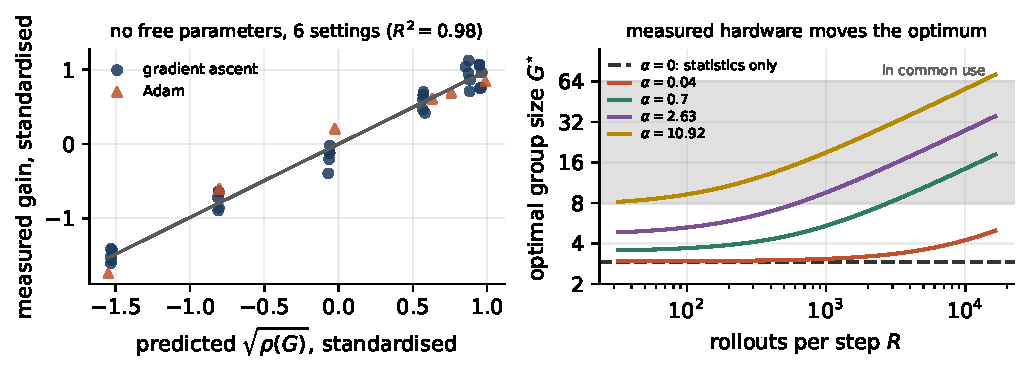
\includegraphics[width=\textwidth]{figures/teaser.pdf}}
    \captionof{figure}{\textbf{Left:} the efficiency $\rho(G)$ predicted from two measured traces
    with no fitted parameters, against the gain actually obtained by training at that split.
    Settings differ in run length and task, so both axes are standardised within a setting; what is
    pooled is the shape. \textbf{Right:} the optimal group size from Theorem~\ref{thm:split} at that
    measured noise ratio, against the rollout budget, for the prefill ratios $\alpha$ we measure on
    real hardware. Statistics alone say three; the hardware says the rest, and says something
    different for long prompts with short answers than for reasoning-length responses.}
    \label{fig:teaser}
  \end{minipage}
  \vspace{10pt}
]

\renewcommand{\thefootnote}{\textdagger}
\footnotetext{ETH Z\"urich neither endorsed nor funded this work. The author was a BSc Computer
Science student throughout this research, which is the source of the affiliation.}
\renewcommand{\thefootnote}{\arabic{footnote}}


\section{Introduction}
\label{sec:introduction}

A paper reports that reinforcement learning post-training moved a benchmark by two points. Whether
that is a result depends on a number nobody has: how much the same procedure would have moved it
had the seed been different. The field is aware of the problem and has documented it
\citep{hochlehnert2025sober}, and the only instrument it has is replication -- run the recipe $N$
times and look at the spread. At the compute scale RLVR now operates at, that instrument is close to
unaffordable, and so the number usually goes unmeasured.

This paper is about what happens between two runs of the same recipe, and it starts from an
observation that turns out to be wrong in a useful way.

If gradient noise perturbs each update and perturbations accumulate, two runs that begin from the
same policy execute a random walk away from each other. Their divergence grows linearly in the
number of updates, a long run is less reproducible than a short one, and the only defence is a
bigger batch. That picture is implicit in how run-to-run variance is discussed, and it is the
natural reading of a noisy gradient.

It does not survive measurement. Two runs which differ only in the randomness of their rollouts
diverge for a few tens of updates and then stop. Across the settings we measure, the log-log slope
of divergence against update count is at most $+0.26$ against the $+1$ a random walk requires, and
usually negative. The runs are climbing the same objective, and its curvature pulls them back
together as fast as the noise pushes them apart. We call this \emph{seed reconvergence}, and its
fixed point is what an error bar on a single run should be built from.

\paragraph{Contributions.}
\begin{itemize}
  \item \textbf{Seed divergence is stationary, not accumulating} (Section~\ref{sec:seeds},
  Section~\ref{sec:experiments}). We measure it on transformers trained from scratch across a
  tenfold range of batch sizes and step sizes, and on a pretrained model, and in no setting that is
  still learning does it accumulate.

  \item \textbf{A law with two measurable factors.}
  $\KL_\infty = \tau_c D_{\mathrm{noise}}$ (Proposition~\ref{prop:stationary}): the diffusive drift
  injected per update, times how long a perturbation survives. It predicts a $P^{-1/2}D^{+1/2}$
  scaling in the batch and the drift, measured at $P^{-0.45}D^{0.35}$ with $R^2 = 0.94$, and an
  outcome spread going as $\sqrt{\KL_\infty}$.

  \item \textbf{An error bar from one run.} $D_{\mathrm{noise}}$ comes from gradients a trainer is
  already accumulating (Section~\ref{sec:estimation}); $\tau_c$ comes from forking the run for a few
  tens of updates rather than repeating it. The alternative currently in use costs $N$ full runs.

  \item \textbf{Where it fails, and why that matters.} A run held to a fixed drift target must raise
  its step size as the objective saturates, because $\E_x[p(1-p)] \to 0$ takes the gradient with it.
  Runs that cross that point leave the contracting regime and separate. The failure is a property of
  drift-targeted control rather than of the law, and it is a caution about a technique this paper
  otherwise recommends.

  \item \textbf{The machinery underneath}, which is of independent use: an exact finite-$G$ mean and
  covariance for the advantage estimators in current use under binary rewards
  (Propositions~\ref{prop:mean} and \ref{prop:cov}). Two things fall out. The estimators differ only
  through a weight $\lambda(p,G)$ on prompt difficulty, so those with a $p$-independent $\lambda$ are
  the same estimator up to a step size. And the gradient noise separates into a between-prompt term
  and a within-prompt term, which is what makes $D_{\mathrm{noise}}$ measurable at all, and which
  incidentally fixes the group size (Theorem~\ref{thm:split}).
\end{itemize}

Every experiment here runs on one laptop. The claim under test is that a small measurement replaces
a large one, and a study that needed a cluster to take the measurement would be a poor advertisement
for it.

\section{Setup}
\label{sec:setup}

A policy $\policy(y \mid x)$ generates a response $y$ to a prompt $x \sim \mathcal{D}$, and a
verifier returns a binary reward $r(x,y) \in \{0,1\}$. The objective is the expected pass rate
\begin{equation}
  J(\theta) = \E_{x} \E_{y \sim \policy(\cdot \mid x)}\big[ r(x,y) \big] = \E_{x}\big[ p(x) \big],
\end{equation}
with $p(x) := \Pr[\, r = 1 \mid x \,]$ the pass rate on prompt $x$.
Write $\score(y) := \nabla_\theta \log \policy(y \mid x)$ for the score, so that
$\E_{y}[\score] = 0$, and let $u_r := \E[\score \mid r]$ and $S_r := \Cov(\score \mid r)$ be the
mean and covariance of the score conditional on the reward. The zero-mean property of the score
gives the identity used throughout,
\begin{equation}
  \label{eq:score-identity}
  p\,u_1 + (1-p)\,u_0 = 0
  \qquad\Longrightarrow\qquad
  u_0 = -\tfrac{p}{1-p}\, u_1 ,
\end{equation}
and the per-prompt gradient is $h(x) := \E_y[r\,\score] = p\, u_1$. Because the reward is binary,
every quantity in this paper depends on the policy only through the four per-prompt objects
$(p, u_1, S_0, S_1)$. That reduction is what makes an exact finite-$G$ theory possible.

\paragraph{Batches.} A batch consists of $P$ prompts drawn independently from $\mathcal{D}$ and $G$
responses drawn independently from the policy for each prompt. We call $G$ the \emph{group size}
and $R = PG$ the \emph{rollouts per step}. Hardware fixes $R$; how to split it is the question.

\paragraph{The estimator family.} Let $k = \sum_{j} r_j$ be the number of successes in a group. We
consider any advantage of the form
\begin{equation}
  \label{eq:family}
  A_j \;=\; w(k, r_j),
\end{equation}
that is, any rule in which a response's advantage depends only on its own reward and on how many
of its group-mates succeeded. This covers the estimators in current use, each of which is fully
described by a $(G+1) \times 2$ table:

\begin{table}[t]
  \centering
  \small
  \begin{tabular}{ll}
    \toprule
    estimator & $w(k, r)$ \\
    \midrule
    RLOO \citep{ahmadian2024rloo} & $r - (k - r)/(G-1)$ \\
    GRPO, mean baseline \citep{liu2025drgrpo} & $r - k/G$ \\
    GRPO, standardised \citep{shao2024deepseekmath}
      & $\dfrac{r - k/G}{\sqrt{(k/G)(1 - k/G)}}$ \\[6pt]
    fixed external baseline & $r - \hat{p}$ \\
    \bottomrule
  \end{tabular}
  \caption{The estimators in current use, each a $(G+1)\times 2$ table. Standardised GRPO is
  defined to be zero when $k \in \{0, G\}$, where the group has no spread.}
  \label{tab:family}
\end{table}

The per-prompt estimator and the batch estimator are
\begin{equation}
  z \;:=\; \frac{1}{G}\sum_{j=1}^{G} w(k, r_j)\, \score(y_j),
  \qquad
  \ghat \;:=\; \frac{1}{P}\sum_{i=1}^{P} z_i .
\end{equation}
Token-level reshaping of the advantage, length normalisation and clipping fall outside
\eqref{eq:family}; Section~\ref{sec:discussion} returns to them.

\section{What the estimators compute, and how noisy they are}
\label{sec:theory}

All results in this section are exact at finite $G$, and all are verified against brute-force
enumeration in Section~\ref{sec:experiments}. Define, for $m \sim \mathrm{Binomial}(G-1, p)$ and
$m' \sim \mathrm{Binomial}(G-2, p)$,
\begin{align}
  \label{eq:contractions}
    W_r &:= \E_m\big[w(r + m, r)\big], \notag \\
  Q_r &:= \E_m\big[w(r + m, r)^2\big], \notag \\
  C_{ab} &:= \E_{m'}\big[w(a + b + m', a)\, w(a + b + m', b)\big].
\end{align}

\subsection{The estimator zoo is a reweighting of prompt difficulty}

\begin{proposition}[Exact expectation]
  \label{prop:mean}
  For any estimator of the form \eqref{eq:family} and any binary reward,
    \begin{equation}
    \E[z \mid x] = \lambda(p, G)\, h(x), \quad \lambda := W_1(p,G) - W_0(p,G).
  \end{equation}
\end{proposition}


Each of the following is exact for every $p$ and every $G$.
RLOO has $W_1 = 1-p$ and $W_0 = -p$, hence $\lambda \equiv 1$: it is unbiased.
GRPO with a mean baseline has $\lambda = (G-1)/G$, independent of $p$: it is RLOO multiplied by a
constant. Standardised GRPO has a $\lambda(p, G)$ with no closed form but an exact binomial sum.

So no member of this family points in the wrong direction. Each computes the true per-prompt
gradient $h(x)$, scaled by a weight that depends on the prompt's difficulty; the family optimises
the reweighted gradient field $\E_x[\lambda(p(x), G)\, h(x)]$, and its members differ only through
$\lambda$. Standardisation is therefore not a variance-reduction device. It is a change of
objective, one that upweights prompts whose pass rate is near $0$ or $1$ relative to prompts of
intermediate difficulty.

A constant $\lambda$ is invisible: rescaling an estimator by $c$ rescales the optimal step size by
$1/c$ and leaves every trajectory unchanged. Only the \emph{dependence of $\lambda$ on $p$} can
alter what a run converges to. This is the sense in which most of the zoo is one estimator.

\subsection{Exact covariance at finite group size}

\begin{proposition}[Exact per-prompt covariance]
  \label{prop:cov}
  With $U := u_1 u_1^{\!\top}$,
  \begin{equation}
    \Cov(z \mid x)
    = \frac{1}{G}\Big[ p\,Q_1 S_1 + (1-p)\,Q_0 S_0 \Big]
    + c_U(p, G)\, U ,
  \end{equation}
    \begin{align}
    c_U &= \frac{1}{G}\Big( p\,Q_1 + \frac{p^2 Q_0}{1-p} \Big) \notag \\
    &\quad + p^2\Big[ \tfrac{G-1}{G}\big( C_{11} - 2C_{10} + C_{00} \big) - \lambda^2 \Big].
  \end{align}
\end{proposition}


\subsection{Two levels of noise}

Prompts are drawn independently, so with $\gbar := \E_x[\lambda h]$ the batch estimator has
\begin{equation}
  \label{eq:hierarchy}
  \Cov(\ghat) \;=\; \frac{1}{P}\Big[ \Sb + \Sw \Big],
\end{equation}
\begin{align}
  \Sb &:= \Cov_x\big( \lambda(p(x), G)\, h(x) \big), \notag \\
  \Sw &:= \E_x\big[ \Cov(z \mid x) \big]. \notag
\end{align}
$\Sb$ is the irreducible variance of sampling prompts and does not shrink with $G$; $\Sw$ is the
variance of sampling responses and does. Pretraining has one level of sampling and therefore one
noise scale. RLVR has two, and the split of a fixed rollout budget between them is a free choice
that nothing in the literature currently determines.

\begin{corollary}[The reward histogram predicts the response-level noise]
  \label{cor:bernoulli}
  For RLOO, $p Q_1 + (1-p) Q_0 = p(1-p)\,G/(G-1)$ exactly, for every $G$. If the conditional score
  covariances are comparable across the two reward classes, $\tr S_0 \approx \tr S_1 \approx
  \sigma_s^2$, then
  \begin{equation}
    \label{eq:bernoulli}
    \tr \Sw \;\approx\; \frac{\sigma_s^2}{G-1}\, \E_x\big[ p(x)\,(1 - p(x)) \big].
  \end{equation}
\end{corollary}

The response-level noise is, up to one slowly varying scalar, the mean Bernoulli variance of the
pass-rate distribution: a quantity every RLVR trainer already logs, at no cost. The isotropy
assumption is measured rather than asserted in Section~\ref{sec:experiments}.

\section{Drift, efficiency, and the optimal split}
\label{sec:drift}

The standard route to a critical batch size is a second-order model of the objective
\citep{mccandlish2018empirical}. For RLVR it is the wrong model. The objective $J = \E[r]$ is not a
log-likelihood, its Hessian is not the negative Fisher information, and along a policy gradient
direction a log-linear policy keeps improving well past the step at which a quadratic model turns
over; measured against exactly computed improvement in Section~\ref{sec:experiments}, it places its
optimum at least four times too low. A model of how far the \emph{policy} moves is accurate over
the same range, and everything below is built on that instead.

\subsection{Drift and efficiency}

One update of size $\eta$ displaces the policy by
\begin{align}
  \label{eq:drift}
  D(\eta) &:= \E_x\Big[ \KL\big( \pi_{t+1}(\cdot \mid x) \,\big\|\, \pi_t(\cdot \mid x) \big) \Big]
  \notag \\
  &\;= \tfrac{1}{2}\eta^2 \big( \mathcal{G} + N/P \big) + O(\eta^3),
\end{align}
with $F$ the Fisher information of the policy, $\mathcal{G} := \gbar^{\!\top} F \gbar$ and
$N := \tr(F\Sb) + \tr(F\Sw)$. In the enumerable testbed this predicts the true KL to within $4\%$
over three orders of magnitude in $\eta$.

Drift splits into a part along the mean update, $\tfrac{1}{2}\eta^2\mathcal{G}$, and a diffusive
part $\tfrac{1}{2}\eta^2 N/P$ that performs a random walk in function space. The fraction that is
signal,
\begin{equation}
  \label{eq:efficiency}
  \rho := \frac{\mathcal{G}}{\mathcal{G} + N/P} = \frac{1}{1 + \Bcrit/P},
  \qquad
  \Bcrit := \frac{N}{\mathcal{G}},
\end{equation}
is the RLVR analogue of the gradient noise scale, measured in prompts. It is a two-level quantity:
a floor set by prompt diversity, plus a term that $G$ divides down. A trainer can therefore read its
own batch-size efficiency off the KL it already logs, without a sweep.

\begin{assumption}[Regularity]
  \label{as:regularity}
  Throughout Section~\ref{sec:drift}: (i) prompts are drawn independently and, given a prompt,
  responses are drawn independently from the current policy; (ii) the advantage rule belongs to the
  count-based family \eqref{eq:family}; (iii) $\tau_w := (G-1)\tr(F\Sw)$ does not depend on $G$,
  which holds exactly for the Bernoulli term of Corollary~\ref{cor:bernoulli} and is measured to
  hold within $6\%$ over $G = 2$ to $32$; (iv) $\eta$ is small enough that the $O(\eta^3)$ term of
  \eqref{eq:drift} is negligible.
\end{assumption}

\subsection{Progress is governed by the square root of the efficiency}

\begin{proposition}[Progress at a fixed drift budget]
  \label{prop:progress}
  Under Assumption~\ref{as:regularity}, let $a := \nabla J^{\!\top}\gbar$ be the alignment of the
  estimator's mean with the true gradient. An update constrained to drift $D$ improves the
  objective, to first order, by
  \begin{equation}
    \label{eq:progress}
    \E[\Delta J] = \sqrt{2D}\;\frac{a}{\sqrt{\mathcal{G}}}\;\sqrt{\rho},
  \end{equation}
  and a run of $N_{\mathrm{s}}$ such updates sharing a total drift budget $D_{\mathrm{tot}}$
  accumulates first-order progress proportional to $\sqrt{N_{\mathrm{s}}\,\rho}$.
\end{proposition}

\begin{proof}
  Solving \eqref{eq:drift} for $\eta$ at drift $D$ gives
  $\eta = \sqrt{2D/(\mathcal{G} + N/P)}$, and the first-order improvement of an update
  $\eta\ghat$ is $\eta\,\E[\ghat]^{\!\top}\nabla J = \eta a$. Substituting and using
  $\rho = \mathcal{G}/(\mathcal{G}+N/P)$ gives \eqref{eq:progress}. Splitting $D_{\mathrm{tot}}$
  equally over $N_{\mathrm{s}}$ updates sets $D = D_{\mathrm{tot}}/N_{\mathrm{s}}$ per update; since
  \eqref{eq:progress} is proportional to $\sqrt{D}$, the total is
  $N_{\mathrm{s}}\sqrt{2D_{\mathrm{tot}}/N_{\mathrm{s}}}\,(a/\sqrt{\mathcal{G}})\sqrt{\rho}
  \propto \sqrt{N_{\mathrm{s}}\rho}$.
\end{proof}

The estimator enters \eqref{eq:progress} only through $a/\sqrt{\mathcal{G}}$, the alignment of
its mean with the true gradient in Fisher units, and the batch composition enters only through
$\rho$. Because KL is quadratic in the step while progress is linear in it, many small
steps travel further than one large step of the same total drift, which is why $N_{\mathrm{s}}$
appears under the square root.

\subsection{The optimal split}

Hardware fixes the rollouts per step $R = PG$; the question is how to divide them. When a group
shares its prompt's prefill, prefill is paid once per prompt and decode once per response, so a step
costs $P(c_{\mathrm{pre}} + G\,c_{\mathrm{dec}})$. Write $\alpha := c_{\mathrm{pre}}/c_{\mathrm{dec}}$
for the prefill ratio and $\beta_b := \tau_b/\mathcal{G}$, $\beta_w := \tau_w/\mathcal{G}$.

\begin{theorem}[Compute-optimal split]
  \label{thm:split}
  Under Assumption~\ref{as:regularity}, maximising the progress of
  Proposition~\ref{prop:progress} per unit of compute at fixed $R$ is equivalent to minimising
  \begin{equation}
    \label{eq:objective}
    f(G) \;=\; (\alpha + G)\Big( \frac{R}{G} + \beta_b + \frac{\beta_w}{G-1} \Big)
  \end{equation}
  over $G \in (1, \infty)$. Then:
  \begin{enumerate}
    \item[(i)] $f$ is strictly convex on $(1,\infty)$ and has a unique minimiser $G^{\star}$, which
    is the unique root of
    \begin{equation}
      \label{eq:stationary}
      \beta_b \;=\; \frac{\alpha R}{G^2} \;+\; \frac{(1+\alpha)\,\beta_w}{(G-1)^2}.
    \end{equation}
    \item[(ii)] If rollouts cost the same however they are grouped $(\alpha = 0)$, then
    \begin{equation}
      \label{eq:gstar}
      G^{\star} \;=\; 1 + \sqrt{\tau_w/\tau_b},
    \end{equation}
    exactly and independently of $R$.
    \item[(iii)] For $\alpha > 0$, $G^{\star}$ is strictly increasing in both $\alpha$ and $R$, and
    \begin{equation}
      \label{eq:gstar-cost}
      G^{\star} \;\to\; 1 + \sqrt{(1+\alpha)\,\tau_w/\tau_b}
      \quad\text{as}\quad \alpha R/G^2 \to 0 .
    \end{equation}
    \item[(iv)] The optimal integer group size is $\lfloor G^{\star}\rfloor$ or
    $\lceil G^{\star}\rceil$.
  \end{enumerate}
\end{theorem}

\begin{proof}
  By Proposition~\ref{prop:progress}, total progress under a compute budget $C$ is proportional to
  $\sqrt{N_{\mathrm{s}}\rho}$ with $N_{\mathrm{s}} = C/\big(P(c_{\mathrm{pre}} + Gc_{\mathrm{dec}})\big)$,
  so
  $N_{\mathrm{s}}\rho \propto \big[(\alpha+G)(P + \Bcrit(G))\big]^{-1}$
  using \eqref{eq:efficiency}. Substituting $P = R/G$ and
  $\Bcrit(G) = \beta_b + \beta_w/(G-1)$ gives \eqref{eq:objective}, and maximising
  $N_{\mathrm{s}}\rho$ is minimising $f$.

  Expanding, $f(G) = \alpha R/G + G\beta_b + (1+\alpha)\beta_w/(G-1) + \text{const}$, whence
  \begin{equation*}
    f''(G) = \frac{2\alpha R}{G^3} + \frac{2(1+\alpha)\beta_w}{(G-1)^3} > 0
    \qquad \text{on } (1,\infty),
  \end{equation*}
  so $f$ is strictly convex. Since $f'(G) \to -\infty$ as $G \downarrow 1$ and
  $f'(G) \to \beta_b > 0$ as $G \to \infty$, $f'$ has a unique zero, which is
  \eqref{eq:stationary}. This proves (i).

  For $\alpha = 0$ the first term of \eqref{eq:stationary} vanishes and the condition reduces to
  $\beta_b = \beta_w/(G-1)^2$, giving \eqref{eq:gstar}; $R$ has dropped out, proving (ii).
  Writing \eqref{eq:stationary} as $\Phi(G,\alpha,R) = 0$ with
  $\Phi := \beta_b - \alpha R/G^2 - (1+\alpha)\beta_w/(G-1)^2$, we have
  $\partial_G \Phi > 0$ at the root while $\partial_\alpha \Phi < 0$ and $\partial_R \Phi < 0$, so
  the implicit function theorem gives $\partial G^{\star}/\partial\alpha > 0$ and
  $\partial G^{\star}/\partial R > 0$. Dropping the $\alpha R/G^2$ term from
  \eqref{eq:stationary} leaves $\beta_b = (1+\alpha)\beta_w/(G-1)^2$, which is
  \eqref{eq:gstar-cost}. This proves (iii). Part (iv) follows from strict convexity, since a
  strictly convex function on an interval is minimised over the integers at one of the two
  integers bracketing its real minimiser.
\end{proof}

Part (ii) is the case in which the split is purely a statistical question, and there the answer is
one plus the square root of the ratio of within-prompt to between-prompt gradient noise, with no
dependence on how many rollouts the hardware affords. Both traces are measurable from a single
batch (Section~\ref{sec:estimation}), so $G^{\star}$ is an observable rather than a hyperparameter.

Part (iii) is where the economics enter, and it is the reason published recipes are not obviously
wrong. Prefill sharing pushes $G^{\star}$ up, and so does a larger rollout budget: a run with long
prompts, short responses and a large batch can have an optimum in the tens even when the purely
statistical optimum is three. Section~\ref{sec:experiments} measures $\alpha$ on real hardware and
finds it ranging from $0.04$ to $10.9$ depending only on the prompt-to-response length ratio, which
moves $G^{\star}$ over an order of magnitude. The approximation \eqref{eq:gstar-cost} that we quote
alongside is the small-batch limit and understates $G^{\star}$ badly when $R$ is large; the root of
\eqref{eq:stationary} is what should be used, and costs one line of arithmetic.

\paragraph{The optimum moves during a run.} Both $\tau_w$ and $\tau_b$ change as the policy
improves. $\E_x[p(1-p)]$ falls once a task is largely solved, while prompt-to-prompt gradient
heterogeneity falls as a model acquires a shared algorithm. Which of the two dominates is an
empirical question, and Section~\ref{sec:experiments} finds both directions in different settings.

\subsection{The step size is a drift target}

Equation \eqref{eq:drift} inverts to $\eta(D) = \sqrt{2D/(\mathcal{G} + N/P)}$, so a run can be
specified by a target drift rather than a learning rate. Learning rate, clip range and KL
coefficient are three controls acting on the single quantity $D$, which is why they interact and why
none of them transfers between settings on its own. Drift is measured in nats per token and is a
property of the policy's behaviour rather than of its parameterisation. Whether that makes it
transfer is tested in Section~\ref{sec:experiments}, and the answer has a boundary.

\section{What happens to two runs that differ only in their seed}
\label{sec:seeds}

Everything so far concerns one update. This section concerns the whole run, and it is where the
noise decomposition earns its keep.

Fix a policy $\theta_0$ and start two runs from it. They see the same prompts and the same
objective, and differ only in the randomness of their rollouts. This is the comparison a
practitioner makes when they change a seed and rerun, and it is the comparison whose spread is
quoted as an error bar when anyone bothers to compute one.

\subsection{The recursion}

Write $\Delta_t := \theta^A_t - \theta^B_t$. With updates $\theta \leftarrow \theta + \eta\ghat$
and $H := \partial\gbar/\partial\theta$ the Jacobian of the mean gradient field,
\begin{equation}
  \label{eq:seed-recursion}
  \Delta_{t+1} = \big( I + \eta H \big)\Delta_t + \eta\,\nu_t,
  \qquad \Cov(\nu_t) = \tfrac{2}{P}\Sigma,
\end{equation}
to first order in $\Delta$, where $\Sigma = \Sb + \Sw$ is the batch noise of
Section~\ref{sec:theory} and the factor of two is because both runs contribute an independent draw.

Equation \eqref{eq:seed-recursion} is a linear stochastic recursion, and its behaviour is decided
by the spectrum of $I + \eta H$. If the objective were flat, $H = 0$, the recursion would be a
random walk: divergence would accumulate, $\E[\|\Delta_t\|^2] \propto t$, and a longer run would be
strictly less reproducible than a short one. That is the implicit model behind treating run-to-run
variance as something to be measured by brute force and reduced only by enlarging the batch.

But two RLVR runs are climbing the same objective. Wherever that objective is locally concave, $H$
is negative definite, $I + \eta H$ is a contraction, and divergence injected at one step decays
over subsequent ones. Whether divergence grows or settles is then a question about which term wins,
and it has an answer.

\subsection{The stationary level}

\begin{proposition}[Stationary seed divergence]
  \label{prop:stationary}
  Suppose $H$ is negative definite with $\eta\lambda_i \ll 1$ for its eigenvalues $-\lambda_i$, and
  that $\Sigma$, $H$ and $\eta$ vary slowly relative to $\max_i 1/(\eta\lambda_i)$. Then
  $\E[\|\Delta_t\|^2]$ converges, and the divergence between the two policies satisfies
  \begin{equation}
    \label{eq:stationary}
    \E\big[\KL(\pi^A \,\|\, \pi^B)\big] \;\longrightarrow\; \tau_c \cdot D_{\mathrm{noise}},
    \qquad
    \tau_c := \frac{1}{\eta\bar\lambda},
  \end{equation}
  where $D_{\mathrm{noise}} = (1-\rho)\,D = \tfrac{1}{2}\eta^2 N/P$ is the diffusive part of the
  drift of Section~\ref{sec:drift} and $\bar\lambda$ is the curvature of the gradient field averaged
  in the Fisher metric.
\end{proposition}

\begin{proof}
  In an eigendirection of $H$ with eigenvalue $-\lambda$, \eqref{eq:seed-recursion} is a scalar
  AR(1) recursion with multiplier $1-\eta\lambda$ and innovation variance $2\eta^2\sigma^2/P$. Its
  stationary variance $c$ solves $c = (1-\eta\lambda)^2 c + 2\eta^2\sigma^2/P$, that is
  $c\,(2\eta\lambda - \eta^2\lambda^2) = 2\eta^2\sigma^2/P$, so $c = \eta\sigma^2/(\lambda P)$ to
  first order in $\eta\lambda$. Summing over directions in the Fisher metric and using
  $\KL \approx \tfrac{1}{2}\Delta^{\!\top} F \Delta$ gives
  $\E[\KL_\infty] = \eta\tr(F\Sigma)/(2\bar\lambda P)$, and substituting
  $D_{\mathrm{noise}} = \tfrac{1}{2}\eta^2\tr(F\Sigma)/P$ yields \eqref{eq:stationary}.
\end{proof}

The statement is worth reading slowly, because each factor is something a trainer can put a number
on. $D_{\mathrm{noise}}$ is how much useless movement one update injects, and
Section~\ref{sec:estimation} recovers it from gradients that are already being accumulated.
$\tau_c$ is how many updates an injected perturbation survives, and it can be had from a short fork
of the run rather than a second full run. Their product is the gap between two seeds.

\subsection{Four predictions}

\eqref{eq:stationary} is falsifiable in four separate ways, and Section~\ref{sec:experiments} tests
each.

\paragraph{Divergence stops growing.} A log-log regression of divergence against update count has
slope $+1$ under the random-walk model and $0$ once \eqref{eq:stationary} is reached.

\paragraph{Run length does not enter.} No $T$ appears in \eqref{eq:stationary}. Training for longer
does not make a run less reproducible, which is not what the random-walk picture would suggest.

\paragraph{The scaling is fixed.} Holding a drift target $D$ rather than a learning rate,
$\eta = \sqrt{2D/(\mathcal{G} + N/P)}$. Below the critical batch size the noise term dominates the
denominator, $\eta \propto \sqrt{DP/N}$, and \eqref{eq:stationary} becomes
\begin{equation}
  \label{eq:seed-scaling}
  \E[\KL_\infty] \;\propto\; P^{-1/2}\, D^{+1/2}.
\end{equation}
Reproducibility improves with the square root of the batch and degrades with the square root of the
step, and depends on nothing else.

\paragraph{Outcome spread follows.} Reading the objective as locally linear in the displacement, the
spread in final task performance across seeds goes as $\sqrt{\E[\KL_\infty]}$.

\subsection{Where the argument stops}

Proposition~\ref{prop:stationary} linearises the gradient field and assumes
$\eta\bar\lambda \ll 1$. Both fail when the step grows relative to the curvature, and there is a
concrete way for that to happen in RLVR: a controller holding drift at a fixed target must raise
$\eta$ as the signal $\mathcal{G}$ decays, and $\mathcal{G}$ decays to zero as a task is solved,
because $\E_x[p(1-p)] \to 0$ takes the gradient with it. A run that saturates while under drift
control therefore drives its own step size up without bound. Section~\ref{sec:experiments} shows
runs crossing out of the contracting regime exactly this way. The law applies while a run is still
learning, which is the regime anyone reports numbers from, and the crossing is a caution about drift
targeting rather than about \eqref{eq:stationary}.

\section{Measuring the two noise scales from a single batch}
\label{sec:estimation}

Both $\tau_b$ and $\tau_w$ are recoverable from gradients a trainer already computes. Index the
microbatches by prompt block and by rollout sub-group and accumulate them separately:
\begin{equation}
  \label{eq:cells}
  g_{ab} := \text{mean gradient over block } a \text{ using sub-group } b,
\end{equation}
for $a = 1 \dots K$ and $b \in \{1,2\}$, each computed with its own sub-group's advantages over
$P/K$ prompts and $G/2$ responses.
Blocks hold disjoint prompts, and given a prompt the two sub-groups are independent, so every term
below is an inner product of independent quantities:
\begin{align}
  \label{eq:estimators}
  \gbar^{\!\top} M \gbar &= \E\big[ g_{a1}^{\!\top} M\, g_{a'2} \big]_{a \neq a'}, \\
  \tr(M\Sb) &= \tfrac{P}{K}\Big( \E\big[ g_{a1}^{\!\top} M\, g_{a2} \big]
     - \gbar^{\!\top} M \gbar \Big), \notag \\
  \tr(M\Sw) &= \tfrac{P}{2K}\, \E\big[ \| g_{a1} - g_{a2} \|_M^2 \big]. \notag
\end{align}
The first pairs different prompts with different responses, the second the same prompts with
different responses, and the third cancels the prompt-level term inside the difference.

The cost is $2K$ gradient buffers rather than one, no extra responses, and no extra backward work
beyond tagging each microbatch -- which any trainer using gradient accumulation is already
positioned to do. Raising $K$ averages the block statistics over $K(K-1)$ ordered pairs rather than
one and shrinks the $P/K$ multiplier in front of the noisiest term, so the estimate improves with
the number of microbatches the trainer already uses. $M = I$ gives the practical form; $M = F$ is
obtained from measured KL rather than by materialising the Fisher.

Getting this right requires handling three biases, each easy to walk into.

\paragraph{The subtractive form is badly conditioned.} Estimating the total variance and
subtracting the within-prompt part differences two large, highly correlated quantities. On
homogeneous pools it returns a negative $\tau_b$ and an infinite $G^{\star}$; where it returns something
finite, it compresses the answer toward the middle of the range. Measured against exactly known
values over pools whose noise ratio spans a factor of $26$, \eqref{eq:estimators} recovers $G^{\star}$
to a median error of $1.3\%$ and a worst case of $6.2\%$, while the subtractive form reports
$6.1$ where the truth is $9.4$ and $6.9$ where the truth is $15.2$.

\paragraph{A repeated prompt lands in two blocks.} Sampling prompts with replacement puts the same
prompt in two blocks, so the different-block inner product picks up a same-prompt term and
$\tau_b$ is biased down -- by $45\%$ on the most homogeneous pool tested. Drawing distinct prompts
within a batch, which iterating a dataset does anyway, removes it.

\paragraph{A finite corpus makes blocks anticorrelated.} Drawing without replacement from a corpus
of $N$ has the opposite effect on the other term: two blocks hold distinct prompts, so
\begin{equation}
  \label{eq:finite-corpus}
  \E\big[ g_{a1}^{\!\top} M\, g_{a'2} \big]_{a \neq a'}
  \;=\; \gbar^{\!\top} M \gbar \;-\; \frac{\tr(M\Sb)}{N-1},
\end{equation}
which is exact and which the estimator corrects using the $\tau_b$ it already has. The correction
matters whenever $\tau_b$ is large relative to the signal -- that is, whenever the run is far below
its critical batch size, which is the usual case. Uncorrected, the signal estimate on one pool came
out negative. The same factor appears in the theory: with a finite corpus the between-prompt
variance enters $\Cov(\ghat)$ multiplied by $1 - (P-1)/(N-1)$, so
\begin{equation}
  \label{eq:gstar-corpus}
  G^{\star} \;=\; 1 + \sqrt{\frac{\tau_w}{\big(1 - \tfrac{P-1}{N-1}\big)\tau_b}},
\end{equation}
and a run that covers its whole corpus every step should use larger groups than one that samples
from a large corpus.

\paragraph{Preconditioners.} An update is $\eta\,\Pi\,\ghat$ for a preconditioner $\Pi$, and Adam
is scale invariant, so both the drift model and the estimators must be read in the metric the
update actually moves in. In practice this means instrumenting the preconditioned gradient: the
results carry over with $F \mapsto \Pi F \Pi$ under the standard assumption that $\Pi$ varies
slowly relative to batch-to-batch fluctuation.

\paragraph{Controlling drift.} Since $D \propto \eta^2$, a multiplicative controller
\begin{equation}
  \eta_{t+1} \;=\; \eta_t \cdot \mathrm{clip}\Big( \big( D^{*} / D_t \big)^{1/2},\ c^{-1},\ c \Big)
\end{equation}
corrects a mis-set step in a single update when the drift estimate is clean. Measured over runs on
transformers, it holds the median drift at its target with no detectable bias in log space.
Exponential smoothing of $D_t$, the obvious refinement, makes it worse: the lag biases the realised
drift low by roughly a factor of two.

\section{Experiments}
\label{sec:experiments}

Three levels of evidence. Policies small enough to enumerate, where the objective, the Fisher
information, the drift and both noise terms are computed rather than estimated. Transformers trained
from scratch, where a population of independent runs executes as one batched kernel so that sweeps
carry standard errors rather than anecdotes. And a pretrained model, where the same measurement is
made on a real policy and a real verifier. Everything ran on a single Apple M4 laptop.

\subsection{Seeds reconverge}
\label{sec:exp-seeds}

A population of transformers is warmed up, given identical parameters, and then trained with each
member drawing its own rollouts. Members differ in nothing else: same prompts corpus, same
objective, same schedule. Divergence is the mean KL between members' policies on a shared batch of
prompts, and outcome spread is the standard deviation of their pass rates, corrected for the
binomial error of the evaluation itself, which at the sample counts normally used accounts for most
of the raw spread and has to be removed before anything can be seen.

\begin{figure*}[t]
  \centering
  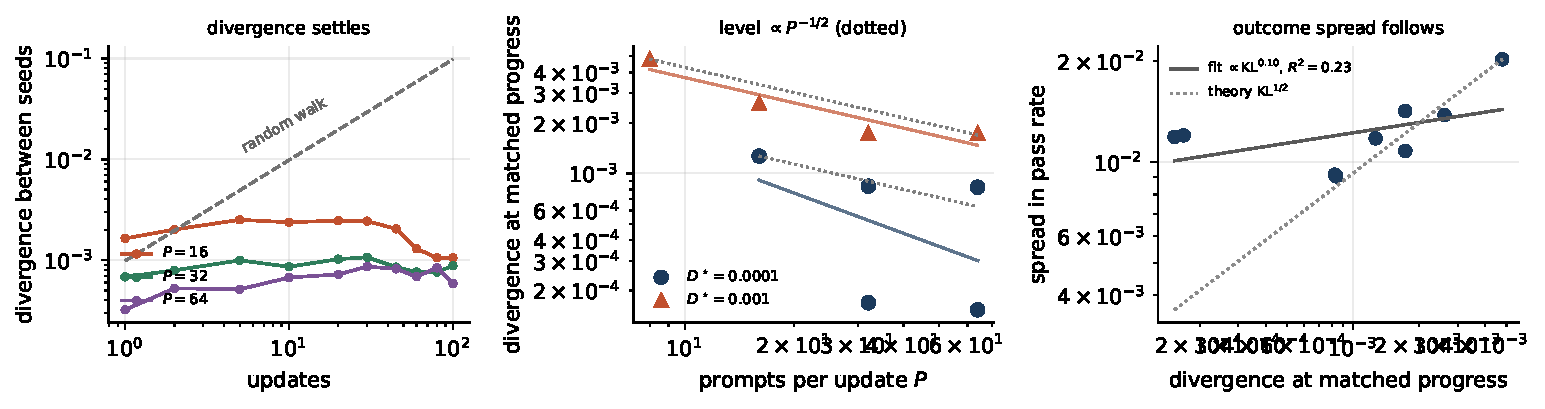
\includegraphics[width=\textwidth]{figures/reconvergence.pdf}
  \caption{\textbf{Left:} divergence between seeds against updates, at a common drift target. The
  dashed line is what an accumulating random walk requires. \textbf{Centre:} the level it settles
  at, compared at matched pass rate rather than matched step count, against the batch; the dotted
  lines are the predicted $P^{-1/2}$. \textbf{Right:} the spread in final pass rate against the
  divergence, one point per setting.}
  \label{fig:reconvergence}
\end{figure*}

\paragraph{It settles.} In every setting that is still learning, divergence rises over the first
few tens of updates and then stops. Fitting a log-log slope over the second half of each run gives
values from $-1.15$ to $+0.26$ across ten settings spanning an eightfold range of batch size and a
tenfold range of drift target, against the $+1$ that accumulation requires. The outcome spread
behaves the same way: it is flat in the number of updates, not growing.

\paragraph{It scales as predicted.} Compared at matched progress, the level follows
$P^{-0.45}D^{0.35}$ against the $P^{-1/2}D^{+1/2}$ of \eqref{eq:seed-scaling}, with $R^2 = 0.94$
over the seven settings where the comparison is available. Both exponents have the right sign and
close to the right magnitude, and the batch is confirmed as the dominant lever: an eightfold
increase in $P$ buys more reproducibility than a tenfold reduction in the step.

\paragraph{What we could not pin down.} \eqref{eq:stationary} factors the level into an injected
noise and a persistence time. The first is measurable; the second is not, at least not the way we
tried. Fitting a single exponential to the approach gives timescales of one to two updates and
predicted levels that miss the measured ones by factors between $1.5$ and $6.6$, with no pattern.
The likely reason is that $H$ has a spectrum rather than one eigenvalue: fast directions equilibrate
immediately and slow ones dominate the final level, so a single-exponential fit is pinned by the
early rise and underestimates what matters. The consequence for practice is a real limitation. The
\emph{scaling} transfers, so a run calibrated once can predict how its reproducibility moves when
the batch or the step changes, which is the question that actually comes up. The absolute level
still requires that one calibration.

\paragraph{Where it stops.} Two of the twelve settings leave the contracting regime, and both do it
the same way. Under a fixed drift target the controller must raise $\eta$ as the signal decays, and
$\E_x[p(1-p)] \to 0$ as a task is solved takes the signal with it. In the two settings that reach a
pass rate above $0.94$, the realised drift runs away to a hundred times its target, divergence jumps
by two orders of magnitude, and the seeds end up in visibly different places: the outcome spread
reaches $0.24$ against $0.01$ elsewhere. This is a failure of drift-targeted control at saturation
rather than of \eqref{eq:stationary}, and it is a caution about a technique we otherwise recommend.

\subsection{Exactly enumerable policies}

The policy is a tabular autoregressive model over a small vocabulary, so its distribution over
sequences, its score at every sequence, and the conditional moments $(p, u_1, S_0, S_1)$ are
available exactly. Propositions~\ref{prop:mean} and~\ref{prop:cov} were checked against
brute-force enumeration over all $|\mathcal{Y}|^{G}$ group outcomes for five estimators and
$G \in \{2,3,4\}$: agreement to $10^{-12}$. The scaled within-prompt term $(G-1)\tr\Sw$, which the
theory treats as $G$-independent, varies by $6\%$ over $G = 2$ to $32$.

\paragraph{The curvature model fails, the drift model does not.} Taking a real update and computing
the resulting improvement and KL exactly, the second-order model of the objective places its optimal
step at least four times below the step that actually maximises improvement, which is where the
sweep ended, because $J = \E[r]$ is
not a log-likelihood and a log-linear policy keeps improving past the turnover of a quadratic model.
The drift model \eqref{eq:drift} predicts the measured KL to between $2.6\%$ and $3.9\%$ across a thousandfold range of step sizes. The theory in Section~\ref{sec:drift} is built on the second of these, not
the first.

\paragraph{Splitting a rollout budget.} For each prompt pool the parameter-free efficiency curve
$\rho(G)$ is compared against the improvement obtained by training at every split of a fixed budget,
holding total rollouts, total drift and step count fixed. Table~\ref{tab:exact-agreement} groups
pools by how much $\rho$ varies across the splits on offer.

\begin{table*}[t]
  \centering
  \begin{tabular}{lccc}
\toprule
predicted spread $\max\rho/\min\rho$ & pools & median $R^2$ & median Spearman \\
\midrule
$1.00$--$1.15$ & 8 & 0.670 & +0.588 \\
$1.15$--$1.35$ & 11 & 0.876 & +0.833 \\
$1.35$--$2.00$ & 6 & 0.971 & +0.957 \\
$2.00$--$8.00$ & 7 & 0.983 & +0.978 \\
\bottomrule
\end{tabular}
  \caption{Agreement between the predicted efficiency and the measured gain in the enumerable
  testbed, as a function of how strongly the prediction discriminates between splits. The prediction
  has no free parameters. Pools where it predicts that the split hardly matters are the pools where
  the measured curves are flat to within their standard errors.}
  \label{tab:exact-agreement}
\end{table*}

\begin{figure*}[t]
  \centering
  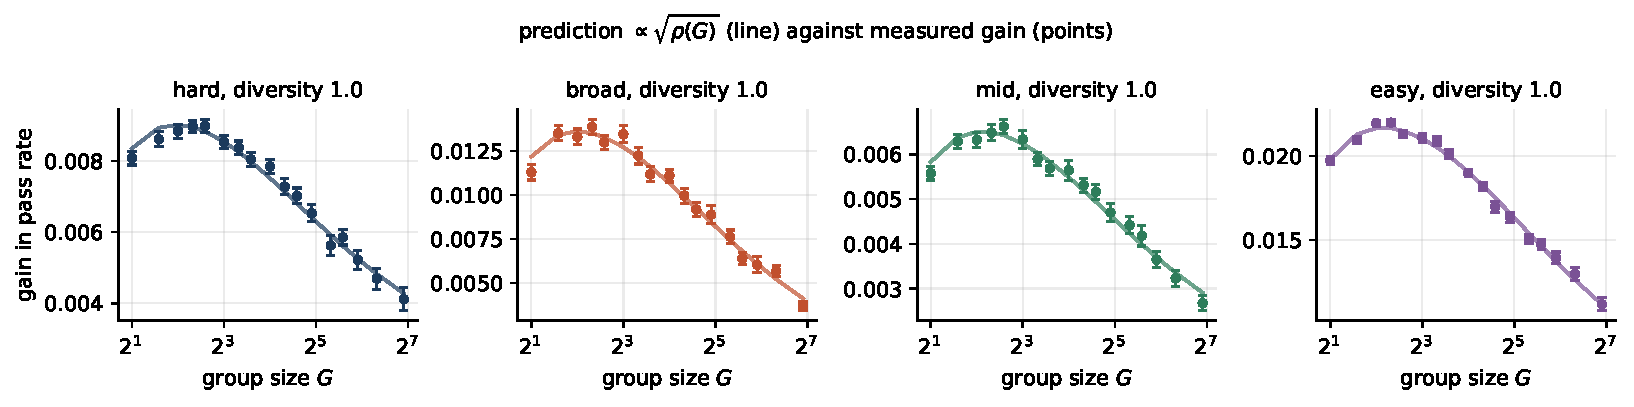
\includegraphics[width=0.98\textwidth]{figures/exact_curves.pdf}
  \caption{Measured gain against $\sqrt{\rho(G)}$ for the four pools whose predictions discriminate
  most strongly. Error bars are standard errors over seeds.}
  \label{fig:exact-curves}
\end{figure*}

\subsection{The estimator}

Figure~\ref{fig:estimator-accuracy} compares the group size recovered by the estimator of
Section~\ref{sec:estimation} against the exactly known value, over pools whose noise ratio spans a
factor of $26$ and whose $G^{\star}$ runs from $3.8$ to $15.2$. The median error in $G^{\star}$ is $1.3\%$
and the worst is $6.2\%$, using $2500$ batches of $32$ prompts split into $K = 8$ blocks; the
individual traces are recovered to $2.1\%$ ($\tau_w$) and $3.4\%$ ($\tau_b$) at the median.

\begin{figure}[t]
  \centering
  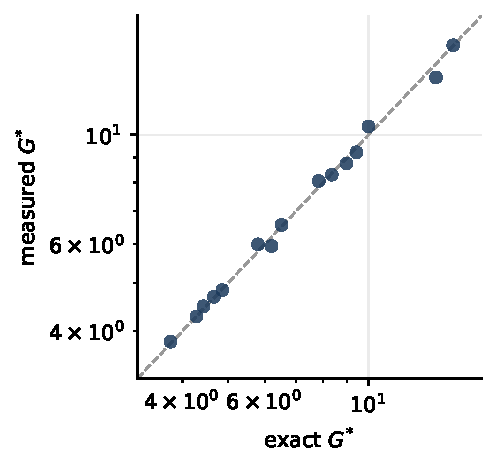
\includegraphics[width=0.92\linewidth]{figures/estimator_accuracy.pdf}
  \caption{Measured against exact optimal group size across prompt pools.}
  \label{fig:estimator-accuracy}
\end{figure}

\subsection{Transformers trained from scratch}

A population of independent transformers is warmed up on a verifiable running-sum task until each
member reaches a common pass rate, the noise terms are measured at that frozen policy, and every
member is then trained from the same starting point at each split of a fixed rollout budget. The
corpus size is the knob: sampling without replacement from a corpus of $N$ scales the between-prompt
term by $1 - (P-1)/(N-1)$, so shrinking the corpus toward the batch raises $G^{\star}$ without touching
the task.

\begin{table*}[t]
  \centering
  \begin{tabular}{lcccccc}
\toprule
corpus $N$ & $\tau_b$ & $\tau_w$ & predicted $G^{\star}$ & best measured $G$ & Spearman & $R^2$ \\
\midrule
128 & 32.1 & 137.1 & 3.38 & 2 & +0.943 & 0.983 \\
192 & 35.4 & 140.3 & 3.17 & 2 & +0.943 & 0.954 \\
512 & 37.6 & 146.8 & 3.04 & 2 & +0.943 & 0.987 \\
4096 & 37.7 & 141.8 & 2.95 & 4 & +1.000 & 0.984 \\
unbounded & 37.3 & 140.0 & 2.94 & 4 & +1.000 & 0.985 \\
\bottomrule
\end{tabular}
  \caption{Predicted and measured optimum on transformers trained from scratch. The sweep visits
  $G \in \{2, 4, 8, 16, 32, 64\}$, so a predicted optimum near three can only appear as a peak at
  two or four; those two are within one standard error of each other in four of the five corpora,
  and every corpus shows the predicted decline beyond $G = 8$. Spearman and $R^2$ are computed
  against the parameter-free prediction across the whole sweep.}
  \label{tab:transformer}
\end{table*}

\begin{figure*}[t]
  \centering
  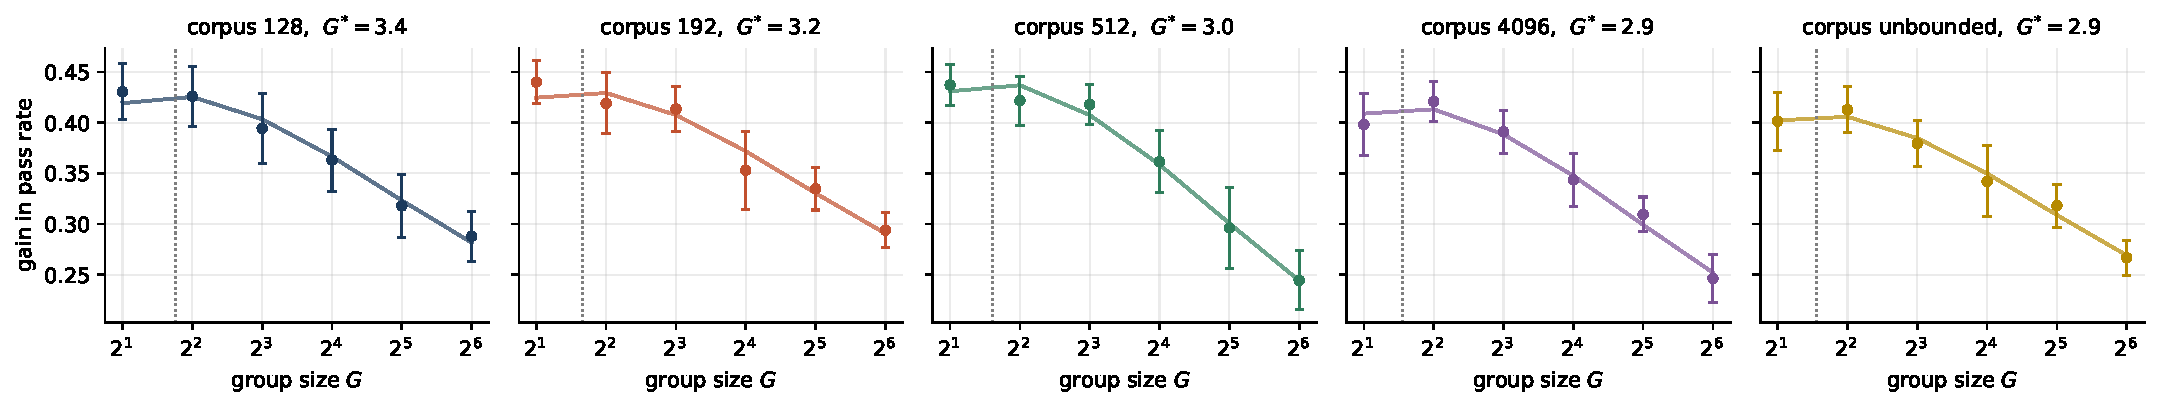
\includegraphics[width=\textwidth]{figures/transformer_curves.pdf}
  \caption{Gain against group size at a fixed rollout budget, with the parameter-free prediction
  overlaid and the predicted $G^{\star}$ marked.}
  \label{fig:transformer-curves}
\end{figure*}

\subsection{Under Adam}
\label{sec:adam}

Everything above is under plain gradient ascent, where the update is the gradient and the noise can
be read in the parameter metric. Real runs use Adam, which moves in a different metric and is scale
invariant, so the theory only carries over if the noise is measured after preconditioning. Repeating
the sweep under both optimisers gives Table~\ref{tab:adam}.

\begin{table*}[t]
  \centering
  \begin{tabular}{lcccccccc}
\toprule
gain by group size & 2 & 4 & 8 & 16 & 32 & 64 & measured $G^{\star}$ & $R^2$ \\
\midrule
gradient ascent & +0.409 & +0.413 & +0.390 & +0.333 & +0.300 & +0.250 & 2.94 & 0.992 \\
Adam & +0.519 & +0.527 & +0.514 & +0.492 & +0.447 & +0.384 & 3.42 & 0.969 \\
\bottomrule
\end{tabular}
  \caption{The same sweep under gradient ascent and under Adam. The optimum is at $G = 4$ for both,
  and the predicted curve explains the measured one about as well. The measured $G^{\star}$ for Adam is
  taken in Adam's own metric, which takes some care -- see below.}
  \label{tab:adam}
\end{table*}

The law survives, but measuring in Adam's metric required fixing two things, and both are
consequences of the preconditioner being an estimated quantity rather than a fixed one.

First, a probe run at a frozen policy starts with an empty second-moment estimate, so there is no
metric to measure in yet. Priming it -- running the optimiser's state forward on real batches with
a zero step size, so the policy does not move -- gives the preconditioner a real run would have.

Second, and less obviously, dividing by $\sqrt{v}$ is unbounded. Coordinates that rarely receive
gradient have a tiny second moment, which is harmless for the update, since Adam's update is
bounded by construction, but ruinous for an inner product between two noisy gradients: those
coordinates dominate it. Measured this way the estimator returned $\tau_b < 0$ and an inverted
efficiency curve. Flooring the second moment at a fraction of its own mean before dividing fixes
it, and the result is insensitive to where the floor is put: over three orders of magnitude in the
floor, the measured $G^{\star}$ moves only from $3.51$ to $3.15$, against an observed optimum of $4$.
Without a floor the same measurement reports $11.9$.

This is the one place where our quantities need care that the plain-gradient case does not. The
working rule is to instrument the update rather than the gradient, and to floor the preconditioner
before inverting it.

\subsection{A pretrained model}

We repeat the measurement on Qwen2.5-0.5B-Instruct with LoRA adapters as the trainable parameters,
over corpora of short exact-match tasks: counting a letter in a word, naming the $k$-th item of a
list, adding two numbers, and a mixture of all of them. Measured optimal group sizes run from $2.7$
to $6.2$, the same range as the enumerable policies and the transformers trained from scratch.

Corollary~\ref{cor:bernoulli} predicts that the within-prompt noise tracks the reward histogram at a
fixed score scale, and difficulty buckets inside one family are where that assumption is tenable.
We screen prompts with a larger sample than the measurement uses, so the bucket boundaries do not
inherit the noise of the quantity under test, and report the pass rate re-measured during the probe
rather than the one used to sort. Across buckets spanning pass rates from $0.25$ to $0.30$, the
ratio $\tau_w/\E[p(1-p)]$ is constant to within $14\%$ (Table~\ref{tab:difficulty}).

\begin{table*}[t]
  \centering
  \small
  \begin{tabular}{lccccc}
\toprule
bucket & screened $p$ & measured $p$ & $\E[p(1-p)]$ & $\tau_w$ & $\tau_w/\E[p(1-p)]$, relative \\
\midrule
0 & 0.160 & 0.253 & 0.163 & 1.15e+04 & 0.90 \\
1 & 0.269 & 0.272 & 0.175 & 1.33e+04 & 0.96 \\
2 & 0.380 & 0.304 & 0.185 & 1.66e+04 & 1.14 \\
\bottomrule
\end{tabular}
  \caption{Within-prompt noise across difficulty buckets of one task family. The gap between the
  screened and re-measured pass rates in the outer buckets is regression to the mean, which is why
  the screening sample is the larger of the two.}
  \label{tab:difficulty}
\end{table*}

Across \emph{different} families the same ratio varies by a factor of $8.8$
(Appendix~\ref{app:cross-family}), and the reason is visible in the assumption: the constant the corollary
predicts is the score scale $\sigma_s^2$, and a family whose answer is one number does not share a
score scale with one whose answer is four. This bounds how the corollary should be used. It
converts a reward histogram into a noise estimate within a task distribution, after one calibration
measurement, and it does not transport that calibration to a task of a different shape.

\subsection{What the hardware is worth}
\label{sec:hardware}

Theorem~\ref{thm:split} turns the split into a question about the serving stack as much as about
the learning problem, through the prefill ratio $\alpha = c_{\mathrm{pre}}/c_{\mathrm{dec}}$. We
measured both costs for a $0.5$B model in bfloat16 on the machine everything else ran on. The ratio
is governed almost entirely by the prompt-to-response length ratio, running from $0.04$ when a
short prompt is followed by a thousand tokens of response to $10.9$ when a thousand-token prompt is
followed by a short answer.

\begin{table*}[t]
  \centering
  \small
  \begin{tabular}{lcccc}
\toprule
$c_{\mathrm{pre}}/c_{\mathrm{dec}}$ & $R=64$ & $R=256$ & $R=1024$ & $R=8192$ \\
\midrule
0.00 & 2.9 & 2.9 & 2.9 & 2.9 \\
0.04 & 3.0 & 3.0 & 3.1 & 4.0 \\
0.70 & 3.6 & 4.0 & 5.5 & 13.1 \\
2.63 & 5.0 & 6.2 & 9.7 & 25.1 \\
10.92 & 8.7 & 11.5 & 19.2 & 51.0 \\
\midrule
\multicolumn{5}{l}{\footnotesize small-batch limit \eqref{eq:gstar-cost} --- $\alpha=0.00$: 2.9, $\alpha=0.04$: 2.9, $\alpha=0.70$: 3.5, $\alpha=2.63$: 4.6, $\alpha=10.92$: 7.6} \\
\bottomrule
\end{tabular}
  \caption{The optimum $G^{\star}$ from Theorem~\ref{thm:split}, at the noise ratio measured on our
  transformers, across measured prefill ratios and rollout budgets. Entries are the root of
  \eqref{eq:stationary}, which agrees with direct numerical minimisation of \eqref{eq:objective} to
  one part in $10^{7}$. The last row shows the small-batch limit, which is what one would quote
  from \eqref{eq:gstar-cost} alone and which understates the optimum badly at large $R$.}
  \label{tab:optimum}
\end{table*}

\begin{figure}[t]
  \centering
  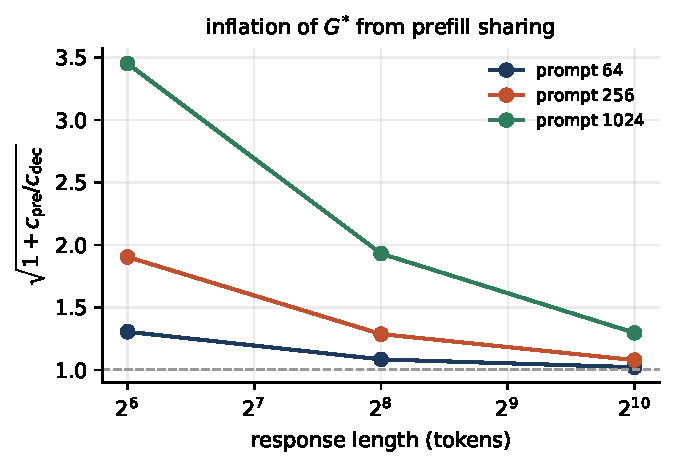
\includegraphics[width=\linewidth]{figures/cost_model.pdf}
  \caption{Measured prefill-to-decode economics on an Apple M4, as the group-size inflation implied
  in the small-batch limit. Long responses make prefill sharing almost worthless; short answers
  behind long prompts make it decisive.}
  \label{fig:cost-model}
\end{figure}

Table~\ref{tab:optimum} is the reconciliation the paper has been building towards. A purely
statistical reading of the split says three; the settings in which published recipes were developed
say otherwise, and the theorem says how much of that is justified. Long prompts with short answers
at a large batch put the optimum in the tens, which is where the recipes are. Reasoning-length
responses, where the response dwarfs the prompt, put it back at three to four, and there a group of
sixteen is spending most of its budget on responses that a second prompt would have used better.
The disagreement between a recipe and this analysis is therefore not evidence against either: it
identifies the regime the recipe came from.

\subsection{What transfers when the batch size changes}

The sharpest consequence of the drift model is a statement about transfer. A run tuned by learning
rate is tuned in a unit that depends on the batch through $\mathcal{G} + N/P$; a run tuned by drift
is not. Table~\ref{tab:transfer} sweeps both parameterisations at four batch sizes and reports what
it costs to carry the value tuned at the smallest batch to the others.

\begin{table*}[t]
  \centering
  \begin{tabular}{lcccc}
\toprule
prompts per step $P$ & 8 & 16 & 32 & 64 \\
\midrule
best step size $\eta^{*}$ & 0.0417 & 0.0786 & 0.1228 & 0.1615 \\
best drift target $D^{*}$ & 5.06e-03 & 5.29e-03 & 5.15e-03 & 3.98e-03 \\
cost of transferring $\eta$ (\%) & +0.0 & -9.9 & -17.9 & -22.0 \\
cost of transferring $D^{*}$ (\%) & +0.0 & +0.0 & +0.0 & +0.0 \\
\bottomrule
\end{tabular}
  \caption{Transfer across batch size. The learning rate that is optimal at $P = 8$ loses a fifth of
  the achievable gain by $P = 64$; the drift target that is optimal at $P = 8$ remains optimal.}
  \label{tab:transfer}
\end{table*}

\begin{figure*}[t]
  \centering
  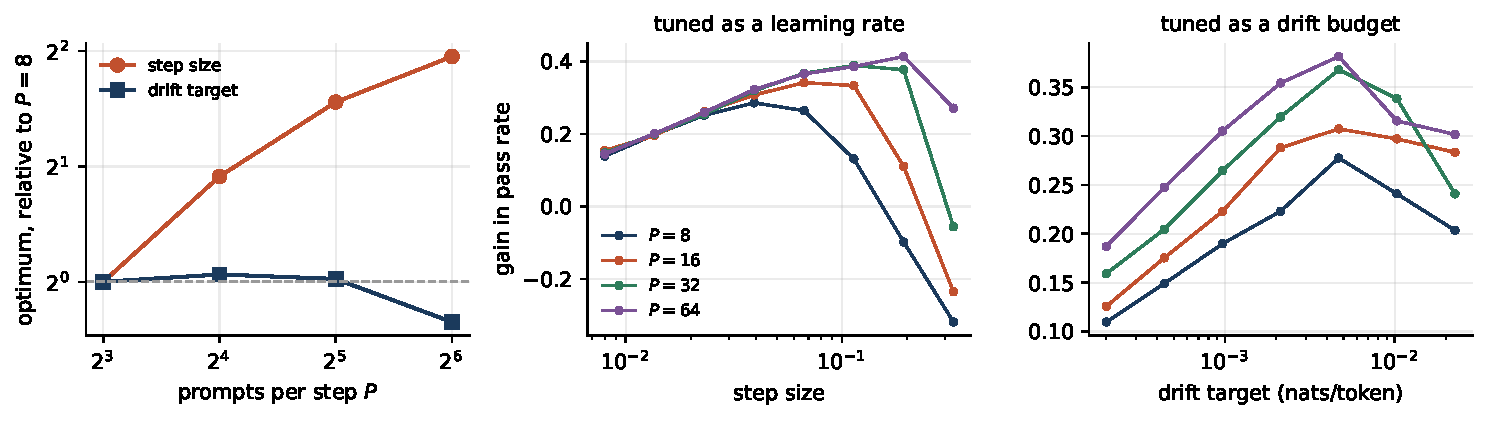
\includegraphics[width=\textwidth]{figures/transfer.pdf}
  \caption{Left: the optimum of each parameterisation relative to its value at $P = 8$. Centre and
  right: the sweeps themselves. The learning-rate optimum moves; the drift optimum does not.}
  \label{fig:transfer}
\end{figure*}

The single-step drift model accounts for part of the movement in $\eta^{*}$ and not all of it: the
coefficient $\mathcal{G} + N/P$ measured at the initial policy predicts a smaller shift than the one
observed over a full run. The coefficient keeps moving as the policy improves, so a controller that re-reads it tracks the
optimum while a learning rate fixed in advance cannot.

\subsection{A prospective test, and where the drift target stops transferring}
\label{sec:recipe}

Everything so far tunes one quantity at a time on the setting it is measured on. The stronger test
is prospective: fix a setting the method has never seen, let the probe choose $G$ before any
training happens, and check afterwards whether it chose well. We moved to a held-out setting with
four times the rollout budget, eight times the corpus and a different seed. The probe reported
$G^{\star} = 3.1$, so the recipe took $G = 4$; the comparison is against $G = 16$, which is what a
default recipe would use.

\begin{table}[t]
  \centering
  \small
  \begin{tabular}{lcc}
\toprule
best achievable gain & $G = 4$ & $G = 16$ \\
\midrule
tuning a learning rate & +0.4947$^{\ast}$ & +0.4780$^{\ast}$ \\
tuning a drift target & +0.4431 & +0.3989 \\
predicted efficiency $\rho$ & 0.815 & 0.674 \\
\bottomrule
\end{tabular}
  \caption{Best achievable gain at the held-out setting, crossing the group size the probe selected
  against the group size a default recipe would use, under both ways of setting the step. Starred
  entries sit at the edge of their grid and are lower bounds. The probe's choice wins under both.}
  \label{tab:diagnosis}
\end{table}

\textbf{The prospective choice was right.} $G = 4$ beats $G = 16$ under both parameterisations.
Under drift control, where the step size is held to the same behavioural budget in both arms and so
cannot confound the comparison, it wins by $11.1\%$ against a predicted
$\sqrt{\rho_4/\rho_{16}} - 1 = 10\%$.

\textbf{The drift target transfers across the group size exactly.} Both group sizes put their
optimum at the same drift target, $1.45 \times 10^{-3}$. Changing how the budget is split does not
change how far the policy should move per update, which is what a behavioural unit ought to do.

\textbf{It does not transfer across this change of budget.} The tuning setting's optimum was
$3.19 \times 10^{-3}$, a factor of $2.2$ away, and carrying it over costs $20\%$ of the achievable
gain. Earlier the same target held to within $5\%$ across a fourfold change in batch size and
$21\%$ across an eightfold one. A sixteenfold change in prompts per step, combined with a fourfold
change in rollout budget, is past where a single number holds. We found this the hard way: packaging
the two together and carrying both to the held-out setting lost to the default by $28.9\%$ (paired
$t = -3.01$ over $32$ runs), and Table~\ref{tab:diagnosis} is what attributes that loss to the drift
target rather than to the group size.

\textbf{A constant drift target is not the right schedule.} At both group sizes a tuned constant
learning rate beat the best constant drift, with its optimum at the edge of the grid. A fixed
learning rate produces a drift that changes over a run as the gradient statistics change, and that
this wins says the optimal drift trajectory is not flat. The unit appears to be right and the
schedule is not, which is the most concrete thing this paper leaves open.

\section{Related work}
\label{sec:related}

\paragraph{Run-to-run variance.} That reinforcement learning results move under reseeding is old
news in deep RL \citep{henderson2018matters} and has been documented again for language-model
reasoning, where sampling parameters, prompt formatting and hardware all shift reported numbers
\citep{hochlehnert2025sober}. Those papers establish the size of the problem by replication, which
is the only instrument available without a model of where the variance comes from. This paper
supplies such a model, and the practical difference is between paying $N$ runs and paying one run
plus a short fork.

\paragraph{Stochastic dynamics of training.} Treating SGD as a stochastic process with a stationary
distribution set by the balance of gradient noise against curvature is standard
\citep{mandt2017sgd}, and the Ornstein-Uhlenbeck argument in Section~\ref{sec:seeds} is that
argument applied to the gap between two runs. What is not established, and what
Section~\ref{sec:experiments} tests, is whether it survives RLVR: the objective is non-stationary
because the data distribution is the policy's own samples, the noise covariance depends on the
pass-rate distribution and moves as the policy improves, and the reward is binary. None of that is
in the setting the original analysis assumes, and the consequence for reproducibility -- that the
spread across seeds does not grow with the length of a run -- does not appear to have been stated
or measured.

\paragraph{Batch size and gradient noise.} The gradient noise scale predicts the batch size beyond
which data parallelism stops buying speed, and does so from statistics measurable during training
\citep{mccandlish2018empirical}; the empirical picture across tasks and optimisers is mapped in
\citet{shallue2019measuring}. Both concern a single level of sampling. RLVR samples prompts and then
samples responses within each prompt, and the resulting two-level noise scale, the split it implies,
and the fact that the response-level term is readable off the reward histogram, have no counterpart
in that literature. The variance decomposition itself is the classical two-stage sampling result
\citep{cochran1977sampling}, applied here to policy gradients.

\paragraph{Hyperparameter transfer.} $\mu$P makes learning rates transfer across width by fixing what
a step does to the network's functions rather than to its parameters
\citep{yang2021tensor, yang2022mutransfer}. This paper takes the same stance one level up: fix what
a step does to the policy's \emph{behaviour}, measured as drift in nats per token, and the recipe
transfers across batch size. We find no comparable prescription for RL post-training in the
literature; the closest work reports empirical scaling behaviour and fitted power laws
\citep{tan2025scalingbehaviors, khatri2025artofscaling, ghosh2026predictable} rather than a
quantity to hold fixed.

\paragraph{Estimators for RLVR.} RLOO \citep{ahmadian2024rloo, williams1992reinforce}, GRPO
\citep{shao2024deepseekmath}, its unnormalised correction \citep{liu2025drgrpo}, DAPO
\citep{yu2025dapo} and sequence-level variants \citep{zheng2025gspo} are usually compared by
benchmark deltas. Proposition~\ref{prop:mean} shows that, for binary rewards, the members of this
family differ only through a difficulty weight $\lambda(p, G)$, that a $p$-independent $\lambda$ is
absorbed exactly by the step size, and that standardisation is a change of objective rather than a
variance reduction -- a sharpening of the argument in \citet{liu2025drgrpo}. Recent analyses of why
normalisation helps \citep{ge2026normalization} and of what outcome-reward objectives cannot
simultaneously be \citep{ding2026impossibility} are complementary: they characterise the estimator,
while the question here is how many samples to give it and how far to step.

\paragraph{Allocating rollouts.} Several recent methods vary the number of responses per prompt
within a batch using heuristics tied to observed pass rates or gradient variance
\citep{nguyen2026allocation}, or adapt the batch size from a divergence signal
\citep{park2026batchscaling}, and one line of work argues for scaling the response count
specifically \citep{hu2025brorl}. These are allocation policies; what has been missing is the
quantity being optimised. Theorem~\ref{thm:split} supplies it, and the answer is a ratio of two measurable traces. This
also explains why heuristics keyed to pass rate alone succeed on some corpora and not others:
the pass rate determines $\tau_w$ and says nothing about $\tau_b$. The two lines of work are
largely orthogonal, since those methods distribute responses across prompts at a group size
someone else chose, while the question here is what that group size should be; the baseline we
compare against is therefore the fixed $G$ of a published recipe rather than an allocation rule.

\paragraph{Trust regions and KL control.} Constraining how far a policy moves is old
\citep{schulman2015trpo, schulman2017ppo} and its modern LLM forms clip importance ratios or
penalise divergence from a reference. The drift used here is neither: it is the KL between
\emph{consecutive} policies, used as a measurement and a control target rather than as a penalty,
and its role in this paper is to supply the unit in which a recipe transfers.

\paragraph{Asynchrony and off-policy correction.} A parallel literature studies what happens when
the sampling policy and the training policy differ, whether through pipeline staleness
\citep{song2026staleness} or numerical mismatch between rollout and training engines. That work
asks how much mismatch a run tolerates. This paper asks a question that arises before any mismatch:
given that the sampler and the trainer agree, how should the sampling budget be divided, and how
large a step should the result support.

\section{Discussion}
\label{sec:discussion}

\paragraph{Group sizes in practice.} Measured on enumerable policies, on transformers trained from
scratch and on a pretrained model, the purely statistical optimum came out between three and six
responses per prompt. Published recipes commonly use eight to sixty-four, and
Theorem~\ref{thm:split}(iii) accounts for the difference without either side being wrong: prefill
sharing and a large rollout budget both push the optimum up, and at the prefill ratios we measure
for long prompts with short answers they push it into the tens. What the theorem removes is the
need to guess. Both inputs are measurements, one from the trainer and one from the serving stack,
and the second changes whenever the prompt-to-response length ratio does.

\paragraph{What the estimator costs.} Four -- or $2K$ -- gradient buffers instead of one, and no
extra responses. A trainer that already accumulates over microbatches gets the decomposition for
the cost of tagging each microbatch with which prompt block and which rollout sub-group it came
from. What it buys is $\Bcrit$, the efficiency $\rho$, and $G^{\star}$, continuously, on the run in
progress rather than from a sweep that has to be repeated when anything changes.

\paragraph{Limits.} The estimator family in \eqref{eq:family} covers advantages that depend on a
response's own reward and its group's success count. It does not cover token-level shaping, length
normalisation, clipping, or a non-binary reward, and the exact moment calculations lean on the
reward being binary. Clipping in particular makes the update a nonlinear function of the batch,
which breaks the linearity the split estimator relies on; it can be handled by instrumenting the
clipped update directly, but the closed forms would need redoing. The drift model is a second-order
expansion and will understate movement for steps large enough to leave that regime. The models measured here run from tabular policies through transformers of $25$k to $400$k
parameters to a pretrained model of $0.5$B, so the claim that these are the right quantities is
tested over four orders of magnitude in parameter count and not beyond; the transfer result is
demonstrated across batch size, not across model scale, where our sweeps were not sharp enough to
separate the two parameterisations.

\paragraph{Preconditioners.} All quantities must be read in the metric the update moves in, and
Section~\ref{sec:adam} shows what that takes in practice: prime the preconditioner before measuring,
and put a floor under its second moment before inverting it, or the coordinates that rarely receive
gradient take over the inner products and the sign of $\tau_b$ stops being reliable. With both in
place the law holds under Adam as well as under gradient ascent. We still treat the preconditioner
as slowly varying relative to batch-to-batch fluctuation, which is standard and which we have not
tested at batch sizes small enough to stress it.

\paragraph{What we would measure next.} Three things. Whether $\tau_w/\tau_b$ moves once responses
are long and reasoning-heavy rather than short and exact-match, since the within-prompt term should
grow with the entropy of the response distribution. How the drift target should be scheduled rather than held constant, since a tuned
constant learning rate beat the best constant drift on the held-out setting of
Section~\ref{sec:recipe}, and whether it transfers across model scale, which needs a sharper
experiment than the one run here. And whether the same decomposition explains the well-known instability of RLVR at small batch
sizes: a run below its critical batch size spends most of its drift budget on diffusion, and the
diffusive fraction is exactly what \eqref{eq:efficiency} measures.

\section*{Use of generative AI}
\addcontentsline{toc}{section}{Use of generative AI}

This work was produced with substantial assistance from a generative AI coding assistant, used
under the author's direction. That assistance covered implementation of the experimental code,
execution and analysis of the experiments, and drafting of this manuscript. The choice of research
direction, the decisions about what to measure and what to discard, and the claims made here are
the author's responsibility.

The disclosure is made because the assistance was not incidental, and two properties of the work
are intended to let a reader check it without reference to how it was produced. Every number
reported in this paper is generated from stored run records by the analysis scripts released
alongside it, rather than transcribed by hand; each record carries the configuration, the commit,
and the platform that produced it. And the analytic results of Sections~\ref{sec:theory} and
\ref{sec:seeds} are checked against brute-force computation by the accompanying test suite, so a
reader who doubts a derivation can run the check rather than re-derive it.


\bibliography{refs}

\appendix
\section{Proofs of the exact moment results}
\label{app:proofs}

\subsection*{Proposition~\ref{prop:mean}}
\begin{proof}
  Condition on $r_j$. The other $G-1$ rewards are i.i.d.\ Bernoulli$(p)$ and, given $r_j$, are
  independent of $\score(y_j)$, so
  $\E[w(k, r_j)\score(y_j)] = \sum_{r} \Pr[r]\, W_r\, u_r$. Summing over $j$ and applying
  \eqref{eq:score-identity} gives $\E[z] = p\,(W_1 - W_0)\,u_1 = \lambda h$.
\end{proof}

\subsection*{Proposition~\ref{prop:cov}}
\begin{proof}
  Split $\E[z z^{\!\top}]$ into diagonal and off-diagonal terms. The diagonal contributes
  $G^{-1}[p Q_1 M_1 + (1-p) Q_0 M_0]$ with $M_r = S_r + u_r u_r^{\!\top}$. For $j \neq l$,
  condition on $(r_j, r_l)$ and on the count $m'$ among the remaining $G-2$ responses; the two
  scores are then conditionally independent, giving
  $\frac{G-1}{G}\sum_{a,b}\Pr[a]\Pr[b]\,C_{ab}\,u_a u_b^{\!\top}$, which collapses to
  $\frac{G-1}{G} p^2 (C_{11} - 2C_{10} + C_{00}) U$ by \eqref{eq:score-identity}. Subtracting
  $\E[z]\E[z]^{\!\top} = \lambda^2 p^2 U$ completes the proof.
\end{proof}

\section{Reproducing the results}
\label{app:repro}

Every figure and table is regenerated from stored run records by
\texttt{analysis/figures.py} and \texttt{analysis/tables.py}; no number in this paper is
transcribed by hand. Each run writes a manifest holding the configuration, its hash, the commit the
code was at, and the interpreter and platform it ran on.

The exactness tests in \texttt{tests/} check every analytic result in Section~\ref{sec:theory}
against brute-force enumeration, and check the batched estimator against the reference
implementation term by term.

\section{The estimator family as a table}
\label{app:family}

Because the advantage depends only on $(k, r)$, an estimator is a $(G+1) \times 2$ array, and the
moments in \eqref{eq:contractions} are contractions of that array against a binomial distribution.
This is what makes the exact treatment cheap: no sampling is involved in evaluating
$\lambda(p, G)$, $Q_r$ or $C_{ab}$ for any member of the family, at any group size.


\section{Noise terms across task families}
\label{app:cross-family}

The corollary relating within-prompt noise to the reward histogram assumes a shared score
scale, which holds within a task family and not between families of different answer shape.
The measurements below make the size of that effect explicit.

\begin{table}[t]
  \centering
  \small
  \begin{tabular}{lcccccc}
\toprule
corpus & pass rate & $\E[p(1-p)]$ & $\tau_b$ & $\tau_w$ & $G^{\star}$ & $\tau_w/\E[p(1-p)]$ \\
\midrule
count letter & 0.280 & 0.178 & 4.35e+02 & 1.16e+04 & 6.15 & 0.27 \\
nth word & 0.326 & 0.138 & 4.88e+03 & 2.01e+04 & 3.03 & 0.61 \\
add two & 0.546 & 0.062 & 1.29e+04 & 3.55e+04 & 2.66 & 2.40 \\
mixed & 0.193 & 0.071 & 4.31e+03 & 1.20e+04 & 2.67 & 0.71 \\
\bottomrule
\end{tabular}
  \caption{Noise terms measured on a pretrained model. The last column would be constant if the
  score scale were shared across families; it is not, and it is not meant to be.}
  \label{tab:real}
\end{table}

\begin{figure}[t]
  \centering
  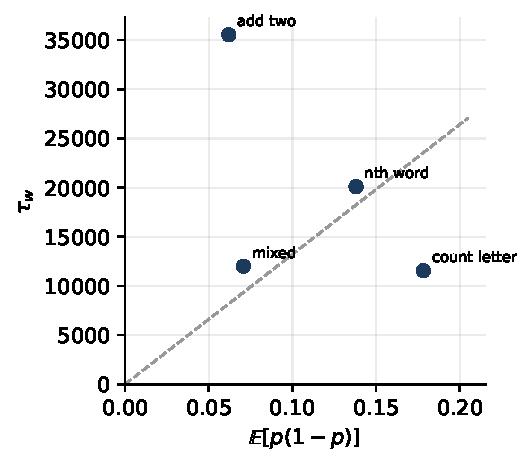
\includegraphics[width=0.95\linewidth]{figures/real_model.pdf}
  \caption{Within-prompt noise against the reward histogram across corpora, with a single fitted
  scale. The scatter is the score scale differing between task families.}
  \label{fig:real-model}
\end{figure}


\end{document}
